\documentclass[12pt]{beamer}

\usepackage[utf8]{inputenc}
\usepackage[frenchb]{babel}
\usepackage{listings,tabu,tikz,amsmath,xcolor,textcomp,framed}

\definecolor{myblue}{rgb}{0,0,0.7}
\definecolor{mygreen}{rgb}{0,0.5,0}
\definecolor{mygray}{rgb}{0.4,0.4,0.4}
\definecolor{mymauve}{rgb}{0.3,0,0.5}
\definecolor{linkblue}{rgb}{0,0.3,0.5}

\newcommand{\urlb}[1]{{\color{linkblue}\url{#1}}}
\newcommand{\hrefb}[2]{{\color{linkblue}\href{#1}{#2}}}

\lstset{
    language=C++, basicstyle=\footnotesize, frame=single,
    literate=%
        {à}{{\`a}}1
        {â}{{\^a}}1
        {É}{{\'E}}1 {é}{{\'e}}1
        {è}{{\`e}}1
        {ê}{{\^e}}1
        {î}{{\^i}}1,
    commentstyle=\color{mygreen},
    keywordstyle=\bf\color{myblue},
    stringstyle=\color{mymauve},
    showstringspaces=false
}

\beamertemplatenavigationsymbolsempty
\AtBeginSection[]
{
    \begin{frame}
    \frametitle{Table des matières}
    \tableofcontents[currentsection]
    \end{frame}
}

\title{Résoudre son premier problème}
\subtitle{UVa 11172 --- Relational Operators}
\author{beOI Training}
\institute{\includegraphics[height=12em]{../share/beoi-logo}}
\date{}

\begin{document}

\maketitle

\begin{frame}
\frametitle{Introduction}
Ce document explique brièvement comment mettre en place l'environnement nécessaire pour programmer et résoudre son premier problème d'algorithmique sur UVa.

~

Les explications se concentrent sur un environnement Linux et l'utilisation de la ligne de commande. Ces outils sont puissants et correspondent aux outils disponibles en concours, donc il est recommandé de savoir un peu les utiliser.

~

Pour utiliser Linux, plusieurs options sont possibles, mais la solution la plus simple pour le début est sans doute de l'installer sur une machine virtuelle. Pour des tutoriels, chercher ``installer ubuntu sur machine virtuelle''\footnote{Certaines instructions dans ce document sont spécifiques à Ubuntu donc si vous n'avez pas d'avis, préférez-le à d'autres distributions de Linux.} sur Google.
\end{frame}


\section{Prérequis}

\edef\hc{\string:}
\begin{frame}
\frametitle{Environnement de programmation (C++)}
Sur Linux:
\begin{itemize}
\item Installer le compilateur g++: \lstinline[language=bash]|sudo apt install g++|
\item Utiliser un bon éditeur de texte: l'éditeur par défaut est parfait (gedit, geany, etc.). Plus avancé: vim, emacs.
\end{itemize}

~

Sur Windows:
\begin{itemize}
\item Meilleure solution: installer Linux (dual boot ou VM)
\item Sinon on conseille Code\hc\hc{}Blocks: \urlb{http://www.codeblocks.org/downloads/binaries}
\item Télécharger le fichier qui ressemble à \texttt{codeblocks-16.01mingw-setup.exe}
\item Ne \textbf{pas} utiliser d'IDE en ligne! (mauvaise habitude)
\end{itemize}
\end{frame}


\begin{frame}
\frametitle{Juges en ligne}
\begin{itemize}
\item Juge en ligne = système qui évalue un code en vérifiant son comportement sur beaucoup d'exemples
\item On va utiliser UVA (il faut créer un compte): \urlb{http://uva.onlinejudge.org}
\end{itemize}
\begin{center}
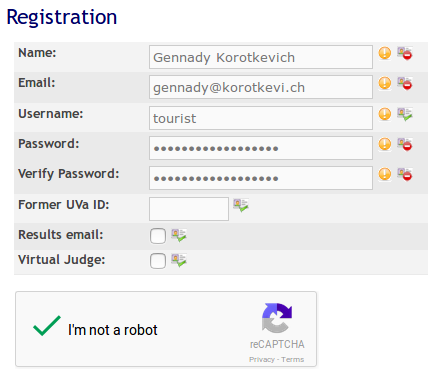
\includegraphics[height=0.45\linewidth]{img/uva-signup}
\end{center}
\end{frame}


\section{Programmation}

\begin{frame}
\frametitle{Introduction du problème}
Énoncé du problème: \urlb{http://uva.onlinejudge.org/external/111/11172.pdf}

\begin{framed}
Some operators checks about the relationship between two values and these operators are called relational operators. \textbf{Given two numerical values} your job is just to \textbf{find out the relationship between them} that is (i) First one is \textbf{greater than} the second (ii) First one is \textbf{less than} the second or (iii) First and second one is \textbf{equal}.
\end{framed}
Lire le contexte en diagonale (un talent à développer).
\end{frame}

\begin{frame}[fragile]
\frametitle{Format d'input}
L'input est donné par l'\emph{entrée standard}, comme si quelqu'un entrait manuellement le fichier ligne par ligne dans la console.

\begin{framed}
\textbf{Input}

First line of the input file is an integer $t$ ($t < 15$) which denotes how many sets of inputs are there.
Each of the next $t$ lines contain two integers $a$ and $b$ ($|a|, |b| < 1000000001$).

~

\textbf{Sample input}\\
\texttt{3\\
10 20\\
20 10\\
10 10
}
\end{framed}
\end{frame}

\begin{frame}[fragile]
\frametitle{Input: test cases}
L'input est très souvent structuré en plusieurs test cases (instances de test) qui se trouvent dans le même fichier.

~

Ici, le nombre de test cases $t$ est donné au début.
\begin{lstlisting}
#include <bits/stdc++.h>
using namespace std;

int main() {
    int t; // nombre de test cases
    cin >> t;
    for (int i=0; i<t; i++) {
        // code ici
    }
}
\end{lstlisting}
\end{frame}

\begin{frame}[fragile]
\frametitle{Input: données}
Il suffit maintenant de lire $a$ et $b$.
\begin{lstlisting}
#include <bits/stdc++.h>
using namespace std;

int main() {
    int t; // nombre de test cases
    cin >> t;
    for (int i=0; i<t; i++) {
        int a,b; // données
        cin >> a >> b;
        // calculer la réponse
    }
}
\end{lstlisting}
Note: \lstinline|cin| permet de lire entiers, flottants et strings, qu'ils soient séparés par des espaces ou des retours à la ligne.
\end{frame}

\begin{frame}[fragile]
\frametitle{Résultat et output}
Maintenant qu'on a $a$ et $b$, il suffit de calculer le résultat.
\begin{lstlisting}
// à l'intérieur de la boucle
if (a < b)
    cout << "<" << endl;
else if (a > b)
    cout << ">" << endl;
else
    cout << "=" << endl;
\end{lstlisting}
Note: Ce n'est pas un problème de commencer à écrire l'output avant d'avoir lu tout l'input.
\end{frame}


\section{Compilation, test, soumission}

\begin{frame}[fragile]
\frametitle{Ouvrir la console}
Les explications pour la compilation et le test vont se concentrer sur un environnement Linux en console.

~

Pour ouvrir la console, deux moyens:
\begin{itemize}
\item L'ouvrir via la liste des applications. Typiquement elle s'appelle ``Terminal'', ``Console'' ou ``Shell''.
\item Depuis l'explorateur de fichier, naviguer vers le dossier puis faire clic droit et ``Open in Terminal'' ou similaire. Avantage: on est directement dans le bon dossier.
\end{itemize}

~

Quand vous ouvrez la console, la ligne qui s'affiche indique le dossier courant: par défaut c'est \lstinline|~|, le dossier ``Home'', qui contient \lstinline|Documents|, \lstinline|Downloads|, ...
\end{frame}

\begin{frame}[fragile]
\frametitle{Commandes de base}
Commandes utiles:
\begin{itemize}
\item \lstinline|ls|: lister le contenu du dossier courant
\item \lstinline|cd dossier|: bouger vers le sous-dossier \lstinline|dossier|
\item \lstinline|cd ..|: revenir dans le dossier parent
\end{itemize}

\begin{center}
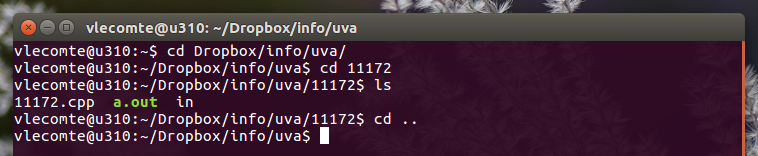
\includegraphics[height=0.17\textwidth]{img/console}
\end{center}

Raccourcis clavier utiles:
\begin{itemize}
\item Tabulation: permet de compléter le nom d'un fichier/dossier/programme partiellement tapé.
\item Flèches haut/bas: permettent de parcourir l'historique et répéter des commandes déjà exécutées.
\end{itemize}
\end{frame}

\begin{frame}[fragile]
\frametitle{Compilation}
Commande pour compiler:
\begin{lstlisting}[language=bash]
g++ -std=c++11 -Wall -Wextra -Wshadow -O2 a.cpp
\end{lstlisting}
\begin{itemize}
\item \lstinline|g++|: nom du compilateur
\item \lstinline|-std=c++11|: version de C++ utilisée
\item \lstinline|-Wall -Wextra -Wshadow|: active plein de warnings très utiles pour écrire des programmes sans bugs
\item \lstinline|-O2|: optimise le programme pour l'accélérer
\item \lstinline|a.cpp|: code source (il faut être dans le bon dossier!)
\end{itemize}
Si tout est ok, ça n'affiche rien et crée le programme \lstinline|a.out|. Sinon, lire les messages d'erreur/warning, corriger et réessayer.

~

Pour changer le nom \lstinline|a.out|, ajouter l'option \lstinline|-o autreNom|.
\end{frame}

\begin{frame}[fragile]
\frametitle{Compilation: pro-tip}
Conseil: ajouter la ligne suivante dans à la fin de \lstinline|~/.bashrc|:
\begin{lstlisting}[language=bash]
alias g="g++ -std=c++11 -Wall -Wextra -Wshadow -O2"
\end{lstlisting}
Le nom \lstinline|.bashrc| commence par un point donc est caché par défaut. Pour l'afficher dans un explorateur de fichier, utiliser Ctrl+H. Il s'ouvre comme un simple fichier texte.
\begin{center}
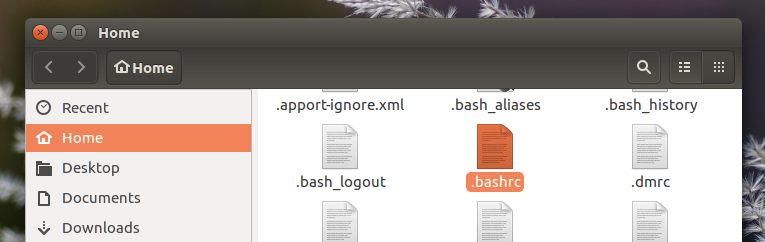
\includegraphics[height=0.2\textwidth]{img/bashrc}
\end{center}

Après redémarrage de la console il suffit de taper \lstinline|g a.cpp| pour compiler avec toutes les options.
\end{frame}

\begin{frame}[fragile]
\frametitle{Test et debugging}
Pour lancer le programme, il suffit de taper \lstinline|./a.out|. Si on donne l'input ligne par ligne, le programme le lira et réagira en conséquence.\footnote{Certains problèmes demandent de lire l'input jusqu'à la ``fin du fichier'' (EOF). Dans ce cas, on peut signaler la fin avec Ctrl+D.}

~

Pour éviter de retaper l'input à chaque fois, on peut le sauver dans un fichier texte (par exemple \lstinline|11172.in|, le nom est sans importance) et le donner au programme automatiquement avec la commande \lstinline|./a.out < 11172.in|. Pour des programmes plus gros, il est recommandé de créer ses propres inputs.

~

De manière similaire, on peut sauver l'output du programme dans un fichier texte avec \lstinline|./a.out > 11172.out| ou même combiner les deux avec \lstinline|./a.out < 11172.in > 11172.out|. Le fichier d'output est créé s'il n'existait pas encore.
\end{frame}

\begin{frame}
\frametitle{Soumission et verdict}
Une fois testé, il est temps de soumettre le programme au juge pour vérifier qu'il est correct et assez rapide. Le plus simple est la page ``Quick Submit'' dans le menu de gauche d'UVa. Entrer le numéro du problème et choisir le langage C++11.

~

Ensuite, on peut voir le verdict dans ``My submissions'':
\begin{itemize}
\item Accepted: le programme est correct, bravo !
\item Wrong Answer: l'output est incorrect
\item Time Limit Exceeded: le programme est trop lent
\item Runtime Error: le programme a crashé
\item Compilation Error: le programme ne compile pas
\item Presentation Error: le format d'output est incorrect
\end{itemize}
\end{frame}

\section{Aller plus loin}

\begin{frame}
\frametitle{Problèmes de sélection beCP}
Maintenant que vous avez résolu votre premier problème, vous pouvez continuer sur le 9 autres problèmes pour la sélection aux stages beCP. Plus d'infos: \urlb{http://becp.be-oi.be/fr/}

~

Après $\sim 1$ jour, vous pourrez utiliser uHunt pour regarder vos statistiques sur UVa: \urlb{http://uhunt.felix-halim.net}
\begin{center}
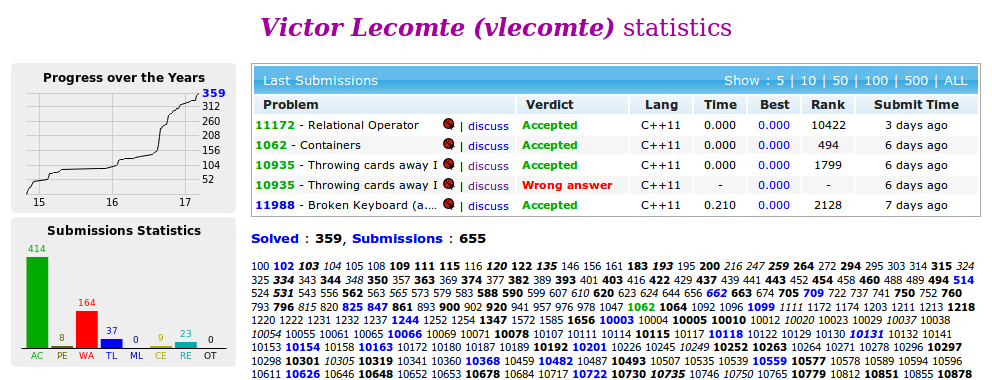
\includegraphics[height=0.3\linewidth]{img/uhunt}
\end{center}
\end{frame}

\begin{frame}
\frametitle{Ressources d'entraînement}
Toutes les ressources d'entraînement beCP sont publiées sur notre site: \urlb{https://github.com/be-oi/beoi-training}
\begin{itemize}
\item Structuré par unités avec des sujets clairement décrits
\item Slides de tous les cours
\item Exercices liés aux sujets vus
\end{itemize}

~

D'autres sites proposent un programme de leçons et exercices assez complet:
\begin{itemize}
\item \hrefb{http://www.france-ioi.org}{France-IOI} (français): site d'entraînement de l'équipe française pour l'IOI.
\item \hrefb{http://train.usaco.org/usacogate}{USACO} (anglais): idem pour les USA.
\end{itemize}
\end{frame}

\begin{frame}
\frametitle{Plateformes et concours}
Il existe de nombreux autres sites avec exercices et concours:
\begin{itemize}
\item \textbf{\hrefb{http://codeforces.com/}{Codeforces}}: bons problèmes et concours réguliers
\item \textbf{\hrefb{https://open.kattis.com/}{Kattis}}: problèmes de qualité, avec indication de niveau\footnote{Il faut parfois prendre des pincettes pour des problèmes qui n'ont pas été résolus par beaucoup d'utilisateurs.}
\item \textbf{\hrefb{http://hsin.hr/coci/}{COCI}}: 7 concours par an, très ciblés IOI
\item \textbf{\hrefb{http://usaco.org}{USACO}}: 4 concours par an, très ciblés IOI, à prendre quand on veut sur un week-end
\item \hrefb{https://www.codechef.com/}{CodeChef}: trois concours par mois dont un sur dix jours
\item \hrefb{https://icpcarchive.ecs.baylor.edu/}{ACM-ICPC Live Archive}: problèmes d'ACM-ICPC, un concours algorithmique universitaire
\item \hrefb{http://www.spoj.com/}{SPOJ}: vaste librairie de problèmes
\end{itemize}
\end{frame}

\begin{frame}
\frametitle{Livres sur l'algorithmique}
Quelques bonnes références sur le competitive programming et l'algorithmique en général:
\begin{itemize}
\item \textbf{\hrefb{https://cses.fi/book.html}{Competitive Programmer's Handbook}} (gratuit): tout nouveau mais a l'air très bien écrit, et assez complet.
\item \hrefb{https://cpbook.net}{Competitive Programming 3} (payant): très complet mais parfois ardu à lire. Inclut des problèmes avec chaque sujet, de qualité variable.
\item \hrefb{http://algs4.cs.princeton.edu/home/}{Algorithms (Sedgewick, Wayne)} (payant): bon livre de référence sur l'algorithmique en général.
\end{itemize}
\end{frame}

\end{document}
